\documentclass[aspectratio=169, 11pt]{beamer}

% ==================== ВЫБОР ЯЗЫКА И КОДИРОВКИ ====================
\usepackage[utf8]{inputenc}
\usepackage[shorthands=off, russian]{babel}
\shorthandoff{"}
\usepackage{amsmath, amsfonts, amssymb, pifont} % Для формул
\usepackage{graphicx} % Для вставки картинок
\usepackage{booktabs} % Для красивых таблиц
\usepackage{csquotes} % Для умных кавычек
\usepackage{hyperref}

% ==================== НАСТРОЙКА ТЕМЫ И ЦВЕТОВ ====================
% Используем тему Madrid как основу (она дает полосу вверху)
\usetheme{Madrid}
% Переопределяем цвета для более современного вида (синий + бирюзовый)
\definecolor{myblue}{RGB}{0, 80, 158}   % Темно-синий
\definecolor{myteal}{RGB}{0, 150, 180}  % Бирюзовый для акцентов

% Устанавливаем цвета элементов
\setbeamercolor{palette primary}{bg=myblue, fg=white}
\setbeamercolor{palette secondary}{bg=myteal, fg=white}
\setbeamercolor{palette tertiary}{bg=myblue!80!black, fg=white}
\setbeamercolor{structure}{fg=myblue} % Цвет маркеров и ссылок
\setbeamercolor{titlelike}{parent=palette primary} % Цвет заголовков

% Убираем навигационные иконки (делает слайды чище)
\setbeamertemplate{navigation symbols}{}

% Делаем точки в оглавлении более круглыми
\setbeamertemplate{section in toc}{\inserttocsectionnumber.~\inserttocsection}

% ==================== НАСТРОЙКА КОЛОНТИТУЛОВ ====================
% Добавляем номер слайда в нижний колонтитул
\setbeamertemplate{footline}{
	\leavevmode%
	\hbox{%
		\begin{beamercolorbox}[wd=\paperwidth,ht=2.25ex,dp=1ex,center]{author in head/foot}%
			\usebeamerfont{author in head/foot}\insertshorttitle\hfill\insertframenumber{} / \inserttotalframenumber
	\end{beamercolorbox}}%
	\vskip0pt%
}

% ==================== РУКОПИСНЫЙ КОД ====================
% Цвета
\definecolor{kw}{RGB}{128,0,128}     % ключевые слова — фиолетовый
\definecolor{tp}{RGB}{0,0,255}       % типы — синий
\definecolor{nm}{RGB}{255,140,0}     % числа — оранжевый
\definecolor{vr}{RGB}{70,90,120}     % переменные — серо-синий
\definecolor{ln}{RGB}{150,150,150}   % номера строк — серый

\newcommand{\K}[1]{\textcolor{kw}{#1}}   % keyword
\newcommand{\T}[1]{\textcolor{tp}{#1}}   % type
\newcommand{\N}[1]{\textcolor{nm}{#1}}   % number
\newcommand{\V}[1]{\textcolor{vr}{#1}}   % variable

% ==================== АННОТАЦИИ ====================
\definecolor{acslkw}{RGB}{128,0,128}   % ключевые слова ACSL (axiomatic, predicate, inductive, case)
\definecolor{acslty}{RGB}{0,0,255}     % типы (float, integer, real, float*)
\definecolor{acslqu}{RGB}{200,0,0}     % кванторы (∀, ∃) — красный
\definecolor{acslid}{RGB}{0,0,0}       % идентификаторы (A, B, C, i, j, k, N, ...)
\definecolor{acslnm}{RGB}{255,140,0}   % числа (0, 1, 0.0)
\definecolor{acsllg}{RGB}{0,128,0}     % логические связки (⟹, ∧, ∨, ≤, ≥)
\definecolor{acslcm}{RGB}{150,150,150} % комментарии
\definecolor{codebg}{RGB}{245,245,245} % фон (уже есть)
\definecolor{acsllb}{RGB}{70,90,120}   % метки

\newcommand{\AK}[1]{\textcolor{acslkw}{#1}}   % ACSL keyword
\newcommand{\AT}[1]{\textcolor{acslty}{#1}}   % type
\newcommand{\AQ}[1]{\textcolor{acslqu}{#1}}   % quantifier
\newcommand{\AI}[1]{\textcolor{acslid}{#1}}   % identifier
\newcommand{\AN}[1]{\textcolor{acslnm}{#1}}   % number
\newcommand{\AL}[1]{\textcolor{acsllg}{#1}}   % logic
\newcommand{\AC}[1]{\textcolor{acslcm}{#1}}   % comment
\newcommand{\ALB}[1]{\textcolor{acsllb}{#1}}  % label
\newcommand{\AS}[1]{\textcolor{acslkw}{#1}}    % assigns / requires / ensures / behavior
\newcommand{\AB}[1]{\textcolor{acslkw}{#1}}    % \nothing, \result, \valid, \valid_read, \separated, \at

\definecolor{abmlat}{RGB}{0,0,0}   % :at — красный
\definecolor{abmlstr}{RGB}{0,128,0}
\newcommand{\AbmlP}[1]{\textcolor{abmlat}{#1}}   % :at
\newcommand{\AbmlS}[1]{\textcolor{abmlstr}{#1}}   % string — зелёный (тот же, что для связок)

% ==================== UNICODE символы ====================
\usepackage{newunicodechar}
\newunicodechar{∀}{\ensuremath{\forall}}
\newunicodechar{∃}{\ensuremath{\exists}}
\newunicodechar{⟹}{\ensuremath{\Rightarrow}}
\newunicodechar{∧}{\ensuremath{\wedge}}
\newunicodechar{∨}{\ensuremath{\vee}}
\newunicodechar{≥}{\ensuremath{\geq}}
\newunicodechar{≤}{\ensuremath{\leq}}
\newunicodechar{×}{\ensuremath{\times}}
\newunicodechar{→}{\ensuremath{\rightarrow}}
\newunicodechar{∈}{\ensuremath{\in}}
\newunicodechar{ℕ}{\ensuremath{\mathbb{N}}}


% ==================== ИНФОРМАЦИЯ О ДОКУМЕНТЕ ====================
\title[Отчет о постановке задач]{Отчет о постановке задач о \\ возможности смены инструмента трансляции на ABML}
\author[Бояндин Лев, Харьков Александр - НГУ]{Бояндин Лев, Харьков Александр - НГУ}
\date{\small{1 октября 2026 г.}}


% ==================== НАЧАЛО ДОКУМЕНТА ====================
\begin{document}


% ==================== ТИТУЛЬНЫЙ СЛАЙД ====================
\begin{frame}[plain]
	\titlepage
\end{frame}


% ==================== ОСНОВНАЯ ЧАСТЬ ====================
\begin{frame}{Поставленные цели}
	Работа пока что проводится только над уже верифицированными версиями программ \\
	(то есть до версии 2 включительно), поскольку сначала необходимо выработать \\
	общую методику на уже проверенных функциях. \\
	\vspace{2em}
	Поставленные цели для подкоманды:
	\begin{itemize}
		\item Цель 1. Выделить присутствующие конструкции языка С;
		\item Цель 2. Построить для этих конструкций онтологию на языке ABML;
		\item Цель 3. Построить аксиоматическую семантику.
	\end{itemize}
\end{frame}


\begin{frame}{Список реализаций}
    Верифицированные реализации алгоритма умножения матриц:
    \vspace{1em}
    \begin{itemize}
        \item Версия 0. Наивная реализация.
        \item Версия 1. С переставленными внутренними циклами.
        \item Версия 2. С интринсиками.
    \end{itemize}
\end{frame}


\begin{frame}[fragile]{Версия 0. Наивная реализация}
	\ttfamily\small
	\setlength{\baselineskip}{1.1em}
	\setlength{\parindent}{0pt}
	
	\begingroup
	\setlength{\fboxsep}{7pt}%
	\colorbox{codebg}{%
		\begin{minipage}{\dimexpr\linewidth-2\fboxsep\relax}
			\begin{tabular}{@{}r@{\hspace{1.2em}}l@{}}
				\textcolor{ln}{1} & \K{void} \V{gemm\_v0}(\T{int} \V{M}, \T{int} \V{N}, \T{int} \V{K}, \T{const} \T{float*} \V{A}, \T{const} \T{float*} \V{B}, \T{float*} \V{C}) \\
				\textcolor{ln}{2} & \{ \\
				\textcolor{ln}{3} & \hspace{2em}\K{for} (\T{int} \V{i} = \N{0}; \V{i} < \V{M}; ++\V{i}) \\
				\textcolor{ln}{4} & \hspace{2em}\{ \\
				\textcolor{ln}{5} & \hspace{4em}\K{for} (\T{int} \V{j} = \N{0}; \V{j} < \V{N}; ++\V{j}) \\
				\textcolor{ln}{6} & \hspace{4em}\{ \\
				\textcolor{ln}{7} & \hspace{6em}\V{C}[\V{i}*\V{N} + \V{j}] = \N{0}; \\
				\textcolor{ln}{8} & \hspace{6em}\K{for} (\T{int} \V{k} = \N{0}; \V{k} < \V{K}; ++\V{k}) \\
				\textcolor{ln}{9} & \hspace{8em}\V{C}[\V{i}*\V{N} + \V{j}] += \V{A}[\V{i}*\V{K} + \V{k}] * \V{B}[\V{k}*\V{N} + \V{j}]; \\
				\textcolor{ln}{10} & \hspace{4em}\} \\
				\textcolor{ln}{11} & \hspace{2em}\} \\
				\textcolor{ln}{12} & \}
			\end{tabular}
		\end{minipage}%
	}%
	\endgroup
\end{frame}


\begin{frame}[fragile]{Версия 1. С переставленными внутренними циклами}
	\ttfamily\small
	\setlength{\baselineskip}{1.1em}
	\setlength{\parindent}{0pt}
	
	\begingroup
	\setlength{\fboxsep}{7pt}%
	\colorbox{codebg}{%
		\begin{minipage}{\dimexpr\linewidth-2\fboxsep\relax}
			\begin{tabular}{@{}r@{\hspace{1.2em}}l@{}}
				\textcolor{ln}{1} & \K{void} \V{gemm\_v1}(\T{int} \V{M}, \T{int} \V{N}, \T{int} \V{K}, \T{const} \T{float*} \V{A}, \T{const} \T{float*} \V{B}, \T{float*} \V{C}) \\
				\textcolor{ln}{2} & \{ \\
				\textcolor{ln}{3} & \hspace{2em}\K{for} (\T{int} \V{i} = \N{0}; \V{i} < \V{M}; ++\V{i}) \\
				\textcolor{ln}{4} & \hspace{2em}\{ \\
				\textcolor{ln}{5} & \hspace{4em}\T{float*} \V{c} = \V{C} + \V{i} * \V{N}; \\
				\textcolor{ln}{6} & \hspace{4em}\K{for} (\T{int} \V{j} = \N{0}; \V{j} < \V{N}; ++\V{j}) \\
				\textcolor{ln}{7} & \hspace{6em}\V{c}[\V{j}] = \N{0}; \\
				\textcolor{ln}{8} & \hspace{4em}\K{for} (\T{int} \V{k} = \N{0}; \V{k} < \V{K}; ++\V{k}) \\
				\textcolor{ln}{9} & \hspace{4em}\{ \\
				\textcolor{ln}{10} & \hspace{6em}\T{const} \T{float*} \V{b} = \V{B} + \V{k} * \V{N}; \\
				\textcolor{ln}{11} & \hspace{6em}\T{float} \V{a} = \V{A}[\V{i}*\V{K} + \V{k}]; \\
				\textcolor{ln}{12} & \hspace{6em}\K{for} (\T{int} \V{j} = \N{0}; \V{j} < \V{N}; ++\V{j}) \\
				\textcolor{ln}{13} & \hspace{8em}\V{c}[\V{j}] += \V{a} * \V{b}[\V{j}]; \\
				\textcolor{ln}{14} & \hspace{4em}\} \\
				\textcolor{ln}{15} & \hspace{2em}\} \\
				\textcolor{ln}{16} & \} \\
			\end{tabular}
		\end{minipage}%
	}%
	\endgroup
\end{frame}


\begin{frame}[fragile]{Версия 2. С интринсиками}
	\ttfamily\footnotesize
	\setlength{\baselineskip}{1.1em}
	\setlength{\parindent}{0pt}
	
	\begingroup
	\setlength{\fboxsep}{7pt}%
	\colorbox{codebg}{%
		\begin{minipage}{\dimexpr\linewidth-2\fboxsep\relax}
			\begin{tabular}{@{}r@{\hspace{1.2em}}l@{}}
				\textcolor{ln}{1} & \K{void} \V{gemm\_v2}(\T{int} \V{M}, \T{int} \V{N}, \T{int} \V{K}, \T{const} \T{float*} \V{A}, \T{const} \T{float*} \V{B}, \T{float*} \V{C}) \\
				\textcolor{ln}{2} & \{ \\
				\textcolor{ln}{3} & \hspace{1.5em}\K{for} (\T{int} \V{i} = \N{0}; \V{i} < \V{M}; ++\V{i}) \\
				\textcolor{ln}{4} & \hspace{1.5em}\{ \\
				\textcolor{ln}{5} & \hspace{3em}\T{float*} \V{c} = \V{C} + \V{i} * \V{N}; \\
				\textcolor{ln}{6} & \hspace{3em}\K{for} (\T{int} \V{j} = \N{0}; \V{j} < \V{N}; \V{j} += \N{8}) \\
				\textcolor{ln}{7} & \hspace{4.5em}\V{\_mm256\_storeu\_ps}(\V{c} + \V{j} + \N{0}, \V{\_mm256\_setzero\_ps}()); \\
				\textcolor{ln}{8} & \hspace{3em}\K{for} (\T{int} \V{k} = \N{0}; \V{k} < \V{K}; ++\V{k}) \\
				\textcolor{ln}{9} & \hspace{3em}\{ \\
				\textcolor{ln}{10} & \hspace{4.5em}\T{const} \T{float*} \V{b} = \V{B} + \V{k} * \V{N}; \\
				\textcolor{ln}{11} & \hspace{4.5em}\V{\_\_m256} \V{a} = \V{\_mm256\_set1\_ps}(\V{A}[\V{i}*\V{K} + \V{k}]); \\
				\textcolor{ln}{12} & \hspace{4.5em}\K{for} (\T{int} \V{j} = \N{0}; \V{j} < \V{N}; \V{j} += \N{16}) \\
				\textcolor{ln}{13} & \hspace{4.5em}\{ \\
				\textcolor{ln}{14} & \hspace{6em}\V{\_mm256\_storeu\_ps}(\V{c} + \V{j} + \N{0}, \V{\_mm256\_fmadd\_ps}(\V{a}, \\
				\textcolor{ln}{15} & \hspace{7.5em}\V{\_mm256\_loadu\_ps}(\V{b} + \V{j} + \N{0}), \V{\_mm256\_loadu\_ps}(\V{c} + \V{j} + \N{0}))); \\
				\textcolor{ln}{16} & \hspace{6em}\V{\_mm256\_storeu\_ps}(\V{c} + \V{j} + \N{8}, \V{\_mm256\_fmadd\_ps}(\V{a}, \\
				\textcolor{ln}{17} & \hspace{7.5em}\V{\_mm256\_loadu\_ps}(\V{b} + \V{j} + \N{8}), \V{\_mm256\_loadu\_ps}(\V{c} + \V{j} + \N{8}))); \\
				\textcolor{ln}{18} & \}\}\}\} \\
			\end{tabular}
		\end{minipage}%
	}%
	\endgroup
\end{frame}


\begin{frame}[fragile]{Спецификация \_mm256\_setzero\_ps}
	\ttfamily\small
	\setlength{\baselineskip}{1.15em}
	\setlength{\parindent}{0pt}
	
	\begingroup
	\setlength{\fboxsep}{0pt}%
	\colorbox{codebg}{%
		\begin{minipage}{\linewidth}
			\vspace{6pt}%
			\hspace{8pt}%
			\begin{tabular}{@{}r@{\hspace{1.2em}}l@{}}
				\textcolor{ln}{1} & \AC{/*@} \\
				\textcolor{ln}{2} & \hspace{2em}\AK{assigns} \AI{\textbackslash nothing}; \\
				\textcolor{ln}{3} & \hspace{2em}\AK{ensures} \AQ{∀} \AT{integer} \AI{i}; \AN{0} \AL{≤} \AI{i} \AL{≤} \AN{7} \AL{⟹} \AI{\textbackslash result}.\AI{e}[\AI{i}] \AL{==} \AN{0.0}; \\
				\textcolor{ln}{4} & \AC{*/} \\
				\textcolor{ln}{5} & \AI{\_\_mm256} \AI{\_mm256\_setzero\_ps}(\AT{void}); \\
			\end{tabular}
			\hspace{8pt}%
			\vspace{4pt}%
		\end{minipage}%
	}%
	\endgroup
\end{frame}


\begin{frame}[fragile]{Спецификация \_mm256\_set1\_ps}
	\ttfamily\small
	\setlength{\baselineskip}{1.15em}
	\setlength{\parindent}{0pt}
	
	\begingroup
	\setlength{\fboxsep}{0pt}%
	\colorbox{codebg}{%
		\begin{minipage}{\linewidth}
			\vspace{6pt}%
			\hspace{8pt}%
			\begin{tabular}{@{}r@{\hspace{1.2em}}l@{}}
				\textcolor{ln}{1} & \AC{/*@} \\
				\textcolor{ln}{2} & \hspace{2em}\AK{assigns} \AI{\textbackslash nothing}; \\
				\textcolor{ln}{3} & \hspace{2em}\AK{ensures} \AQ{∀} \AT{integer} \AI{i}; \AN{0} \AL{≤} \AI{i} \AL{≤} \AN{7} \AL{⟹} \AI{\textbackslash result}.\AI{e}[\AI{i}] \AL{==} \AI{v}; \\
				\textcolor{ln}{4} & \AC{*/} \\
				\textcolor{ln}{5} & \AI{\_\_mm256} \AI{\_mm256\_set1\_ps}(\AT{float} \AI{v}); \\
			\end{tabular}
			\hspace{8pt}%
			\vspace{4pt}%
		\end{minipage}%
	}%
	\endgroup
\end{frame}


\begin{frame}[fragile]{Спецификация \_mm256\_loadu\_ps}
	\ttfamily\small
	\setlength{\baselineskip}{1.15em}
	\setlength{\parindent}{0pt}
	
	\begingroup
	\setlength{\fboxsep}{0pt}%
	\colorbox{codebg}{%
		\begin{minipage}{\linewidth}
			\vspace{6pt}%
			\hspace{8pt}%
			\begin{tabular}{@{}r@{\hspace{1.2em}}l@{}}
				\textcolor{ln}{1} & \AC{/*@} \\
				\textcolor{ln}{2} & \hspace{2em}\AK{requires} \AI{\textbackslash valid\_read}(\AI{a} \AL{+} (\AN{0} \AL{..} \AN{7})); \\
				\textcolor{ln}{3} & \hspace{2em}\AK{assigns} \AI{\textbackslash nothing}; \\
				\textcolor{ln}{4} & \hspace{2em}\AK{ensures} \AQ{∀} \AT{integer} \AI{i}; \AN{0} \AL{≤} \AI{i} \AL{≤} \AN{7} \AL{⟹} \AI{\textbackslash result}.\AI{e}[\AI{i}] \AL{==} \AI{a}[\AI{i}]; \\
				\textcolor{ln}{5} & \AC{*/} \\
				\textcolor{ln}{6} & \AI{\_\_mm256} \AI{\_mm256\_loadu\_ps}(\AT{const} \AT{float*} \AI{a}); \\
			\end{tabular}
			\hspace{8pt}%
			\vspace{4pt}%
		\end{minipage}%
	}%
	\endgroup
\end{frame}


\begin{frame}[fragile]{Спецификация \_mm256\_storeu\_ps}
	\ttfamily\small
	\setlength{\baselineskip}{1.15em}
	\setlength{\parindent}{0pt}
	
	\begingroup
	\setlength{\fboxsep}{0pt}%
	\colorbox{codebg}{%
		\begin{minipage}{\linewidth}
			\vspace{6pt}%
			\hspace{8pt}%
			\begin{tabular}{@{}r@{\hspace{1.2em}}l@{}}
				\textcolor{ln}{1} & \AC{/*@} \\
				\textcolor{ln}{2} & \hspace{2em}\AK{requires} \AI{\textbackslash valid}(\AI{mem\_addr} \AL{+} (\AN{0} \AL{..} \AN{7})); \\
				\textcolor{ln}{3} & \hspace{2em}\AK{assigns} \AI{mem\_addr}[\AN{0} \AL{..} \AN{7}]; \\
				\textcolor{ln}{4} & \hspace{2em}\AK{ensures} \AQ{∀} \AT{integer} \AI{i}; \AN{0} \AL{≤} \AI{i} \AL{≤} \AN{7} \AL{⟹} \AI{mem\_addr}[\AI{i}] \AL{==} \AI{a}.\AI{e}[\AI{i}]; \\
				\textcolor{ln}{5} & \AC{*/} \\
				\textcolor{ln}{6} & \AK{void} \AI{\_mm256\_storeu\_ps}(\AT{float*} \AI{mem\_addr}, \AI{\_\_mm256} \AI{a}); \\
			\end{tabular}
			\hspace{8pt}%
			\vspace{4pt}%
		\end{minipage}%
	}%
	\endgroup
\end{frame}


\begin{frame}[fragile]{Спецификация \_mm256\_fmadd\_ps}
	\ttfamily\small
	\setlength{\baselineskip}{1.15em}
	\setlength{\parindent}{0pt}
	
	\begingroup
	\setlength{\fboxsep}{0pt}%
	\colorbox{codebg}{%
		\begin{minipage}{\linewidth}
			\vspace{6pt}%
			\hspace{8pt}%
			\begin{tabular}{@{}r@{\hspace{1.2em}}l@{}}
				\textcolor{ln}{1} & \AC{/*@} \\
				\textcolor{ln}{2} & \hspace{2em}\AK{assigns} \AI{\textbackslash nothing}; \\
				\textcolor{ln}{3} & \hspace{2em}\AK{ensures} \AQ{∀} \AT{integer} \AI{i}; \AN{0} \AL{≤} \AI{i} \AL{<} \AN{8} \\
				\textcolor{ln}{3} & \hspace{2em}\AL{⟹} \AI{\textbackslash result}.\AI{e}[\AI{i}] \AL{==} \AI{a}.\AI{e}[\AI{i}] \AL{*} \AI{b}.\AI{e}[\AI{i}] \AL{+} \AI{c}.\AI{e}[\AI{i}]; \\
				\textcolor{ln}{4} & \AC{*/} \\
				\textcolor{ln}{5} & \AI{\_\_mm256} \AI{\_mm256\_fmadd\_ps}(\AI{\_\_mm256} \AI{a}, \AI{\_\_mm256} \AI{b}, \AI{\_\_mm256} \AI{c}); \\
			\end{tabular}
			\hspace{8pt}%
			\vspace{4pt}%
		\end{minipage}%
	}%
	\endgroup
\end{frame}


\begin{frame}{Что такое ABML?}
	Предметно-ориентированный язык программирования ABML (Attribute-Based Modeling Language) - это лексическое расширение Common Lisp.
	\vspace{2em}
	
	\ttfamily\small
	\setlength{\baselineskip}{1.1em}
	\setlength{\parindent}{0pt}
	
	\begingroup
	\setlength{\fboxsep}{7pt}%
	\colorbox{codebg}{%
		\begin{minipage}{\dimexpr\linewidth-2\fboxsep\relax}
			\begin{tabular}{@{}r@{\hspace{1.2em}}l@{}}
				\textcolor{ln}{1} & \K{for} (\T{int} \V{i} = \N{0}; \V{i} < \V{M}; ++\V{i}) \{ \\
				\textcolor{ln}{2} & \hspace{2em} \AC{// Какое-то тело цикла} \\
				\textcolor{ln}{3} & \} \\
			\end{tabular}
		\end{minipage}%
	}%
	\endgroup
\end{frame}


\begin{frame}[fragile]{ABML: пример онтологии}
	\ttfamily\small
	\setlength{\baselineskip}{1.15em}
	\setlength{\parindent}{0pt}
	
	\begingroup
	\setlength{\fboxsep}{0pt}%
	\colorbox{codebg}{%
		\begin{minipage}{\linewidth}
			\vspace{6pt}%
			\hspace{8pt}%
			\begin{tabular}{@{}r@{\hspace{1.2em}}l@{}}
				\textcolor{ln}{1} & (\AK{typedef} \AbmlS{"type"} (\AI{uniont} \AbmlS{"int type"})) \\
				\textcolor{ln}{2} & (\AK{cot} \AbmlS{"int type"}) \\
				\textcolor{ln}{3} & \\
				\textcolor{ln}{4} & (\AK{typedef} \AbmlS{"variable name"} \AT{string}) \\
				\textcolor{ln}{5} & (\AK{mot} \AbmlS{"variable acces"} \AbmlP{:at} \AN{1} \AbmlS{"variable name"}) \\
				\textcolor{ln}{6} & (\AK{mot} \AbmlS{"cell"} \AbmlP{:at} \AbmlS{"type"} \AbmlS{"type"} \AbmlP{:at} \AbmlS{"value"} \AbmlS{"C value"}) \\
				\textcolor{ln}{7} & \\
				\textcolor{ln}{8} & (\AK{typedef} \AbmlS{"expression"} (\AI{uniont} \AbmlS{"C value"} \AbmlS{"variable acces"} \AbmlS{"1<2"})) \\
				\textcolor{ln}{9} & (\AK{typedef} \AbmlS{"C value"} (\AI{uniont} \AT{bool} \AT{int} \AT{real})) \\
				\textcolor{ln}{10} & (\AK{mot} \AbmlS{"1<2"} \AbmlP{:at} \AN{1} \AbmlS{"C value"} \AbmlP{:at} \AN{2} \AbmlS{"C value"}) \\
				\textcolor{ln}{11} & \\
				\textcolor{ln}{12} & (\AK{typedef} \AbmlS{"statement"} (\AI{uniont} \AbmlS{"++1"} \AbmlS{"for stmt"})) \\
				\textcolor{ln}{13} & (\AK{cot} \AbmlS{"++1"} \AbmlP{:at} \AN{1} \AbmlS{"variable name"}) \\
				\textcolor{ln}{14} & (\AK{mot} \AbmlS{"for stmt"} \AbmlP{:at} \AbmlS{"init"} \AbmlS{"statement"} \AbmlP{:at} \AbmlS{"condition"} \AbmlS{"expression"} \\
				\textcolor{ln}{15} & \hspace{8em}\AbmlP{:at} \AbmlS{"post"} \AbmlS{"statement"} \AbmlP{:at} \AbmlS{"body"} \AbmlS{"block"}) \\
				\textcolor{ln}{16} & \\
				\textcolor{ln}{17} & (\AK{mot} \AbmlS{"block"} \AbmlP{:at} \AbmlS{"sts"} (\AI{listt} \AbmlS{"statement"})) \\
			\end{tabular}
			\hspace{8pt}%
			\vspace{4pt}%
		\end{minipage}%
	}%
	\endgroup
\end{frame}

\iffalse
\begin{frame}[fragile]{Пример на языке C: два варианта цикла}
	
	% ---------- Блок 1 ----------
	\textbf{Вариант 1:} переменная объявлена прямо в заголовке \texttt{for}.
	
	\vspace{0.3em}
	
	\begingroup
	\setlength{\fboxsep}{0pt}%
	\colorbox{codebg}{%
		\begin{minipage}{\linewidth}
			\ttfamily\small
			\setlength{\baselineskip}{1.15em}
			\vspace{6pt}%
			\hspace{8pt}%
			\begin{tabular}{@{}r@{\hspace{1.2em}}l@{}}
				\textcolor{ln}{1} & \K{for} (\T{int} \V{i} = \N{0}; \V{i} < \N{9}; ++\V{i}) \{ \AL{...} \} \\
			\end{tabular}
			\hspace{8pt}%
			\vspace{4pt}%
		\end{minipage}%
	}%
	\endgroup
	
	\vspace{2em}
	
	% ---------- Блок 2 ----------
	\textbf{Вариант 2:} переменная объявлена заранее, в \texttt{for} пустая инициализация.
	
	\vspace{0.3em}
	
	\begingroup
	\setlength{\fboxsep}{0pt}%
	\colorbox{codebg}{%
		\begin{minipage}{\linewidth}
			\ttfamily\small
			\setlength{\baselineskip}{1.15em}
			\vspace{6pt}%
			\hspace{8pt}%
			\begin{tabular}{@{}r@{\hspace{1.2em}}l@{}}
				\textcolor{ln}{1} & \{ \\
				\textcolor{ln}{2} & \hspace{2em}\T{int} \V{i} = \N{0}; \\
				\textcolor{ln}{3} & \hspace{2em}\K{for} (; \V{i} < \N{9}; ++\V{i}) \{ \AL{...} \} \\
				\textcolor{ln}{4} & \} \\
			\end{tabular}
			\hspace{8pt}%
			\vspace{4pt}%
		\end{minipage}%
	}%
	\endgroup
\end{frame}
\fi


\begin{frame}{Визуализация умножения матриц}
	\begin{center}
		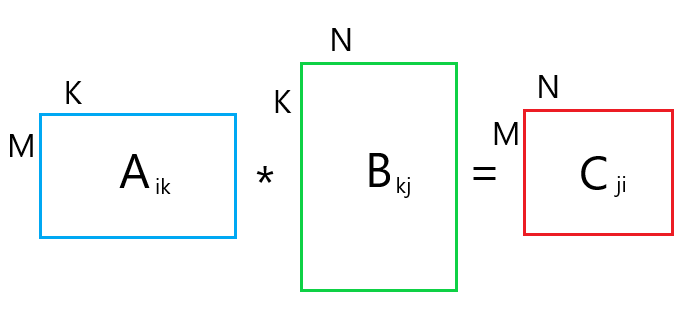
\includegraphics[scale=0.8]{img/matrix_mult.png}
	\end{center}
\end{frame}


\end{document}
